%===============================================================================================
%		Reference Examples
%===============================================================================================

\chapter{Reference Examples}
\label{sec:ReferenceExamples}

To proof conformance with the \LibName{} requirements, a set of (mostly) real-life examples for all supported formats is used. The examples are used to illustrate design decisions and also to verify them. In this chapter, these examples are presented for short. The concrete detailed structures of each data format is described in \cite{MetadataCompendium}.

Note that the sizes of the data blocks in the following illustrating example figures do not have any specific meaning.

%-----------------------------------------------------------------------------------------------
%		Example 1: MP3 File with ID3v2.3 and ID3v1.1
%-----------------------------------------------------------------------------------------------

\section{Example 1: MP3 File with ID3v2.3, ID3v1.1 and Lyrics3}
\label{sec:Example1MP3FileWithID3v23AndID3v11}

The following figure shows the first example, an MP3 file with three \TERMtag{}s, ID3v2.3, Lyrics3v2 and ID3v1.1. All are located at the end of the file:

\begin{figure}[H]
	\centering
	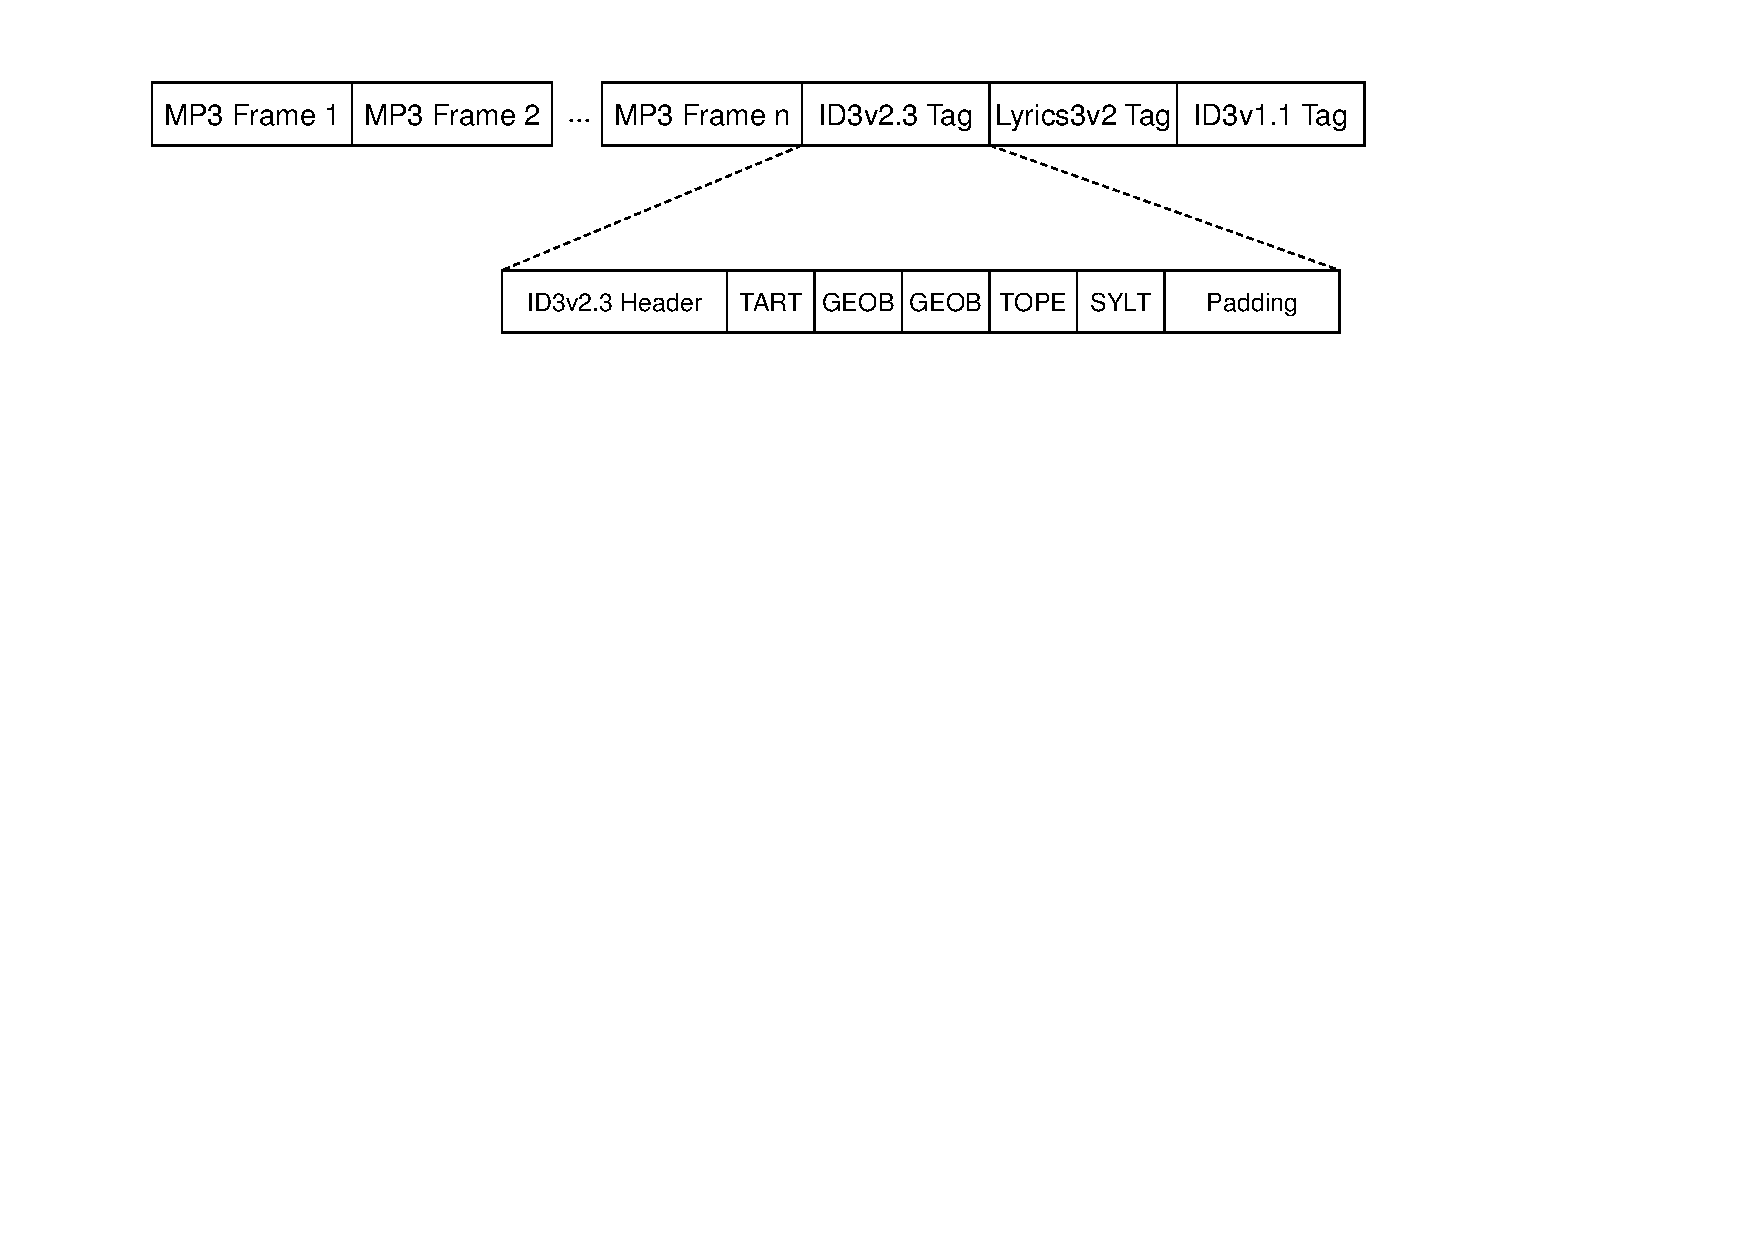
\includegraphics[width=1.00\textwidth]{Figures/Part_I/I_5_Example1.pdf}
	\caption{Example 1: MP3 file with two tags}
	\label{fig:Example1MP3filewithtwotags}
\end{figure}

The ID3v2.3 tag has several frames, including two \texttt{GEOB} frames. Furthermore, it has some padding within. Each of the MP3 frames corresponds to the MPEG-1 elementary stream audio format.

%-----------------------------------------------------------------------------------------------
%		Example 2: MP3 File with two ID3v2.4 Tags
%-----------------------------------------------------------------------------------------------

\section{Example 2: MP3 File with two ID3v2.4 Tags}
\label{sec:Example2MP3FileWithID3v23AndID3v11}

The following figure shows the second example, an MP3 file with two ID3v2.4 \TERMtag{}s, one at the beginning, the other one at the end of the file:

\begin{figure}[H]
	\centering
	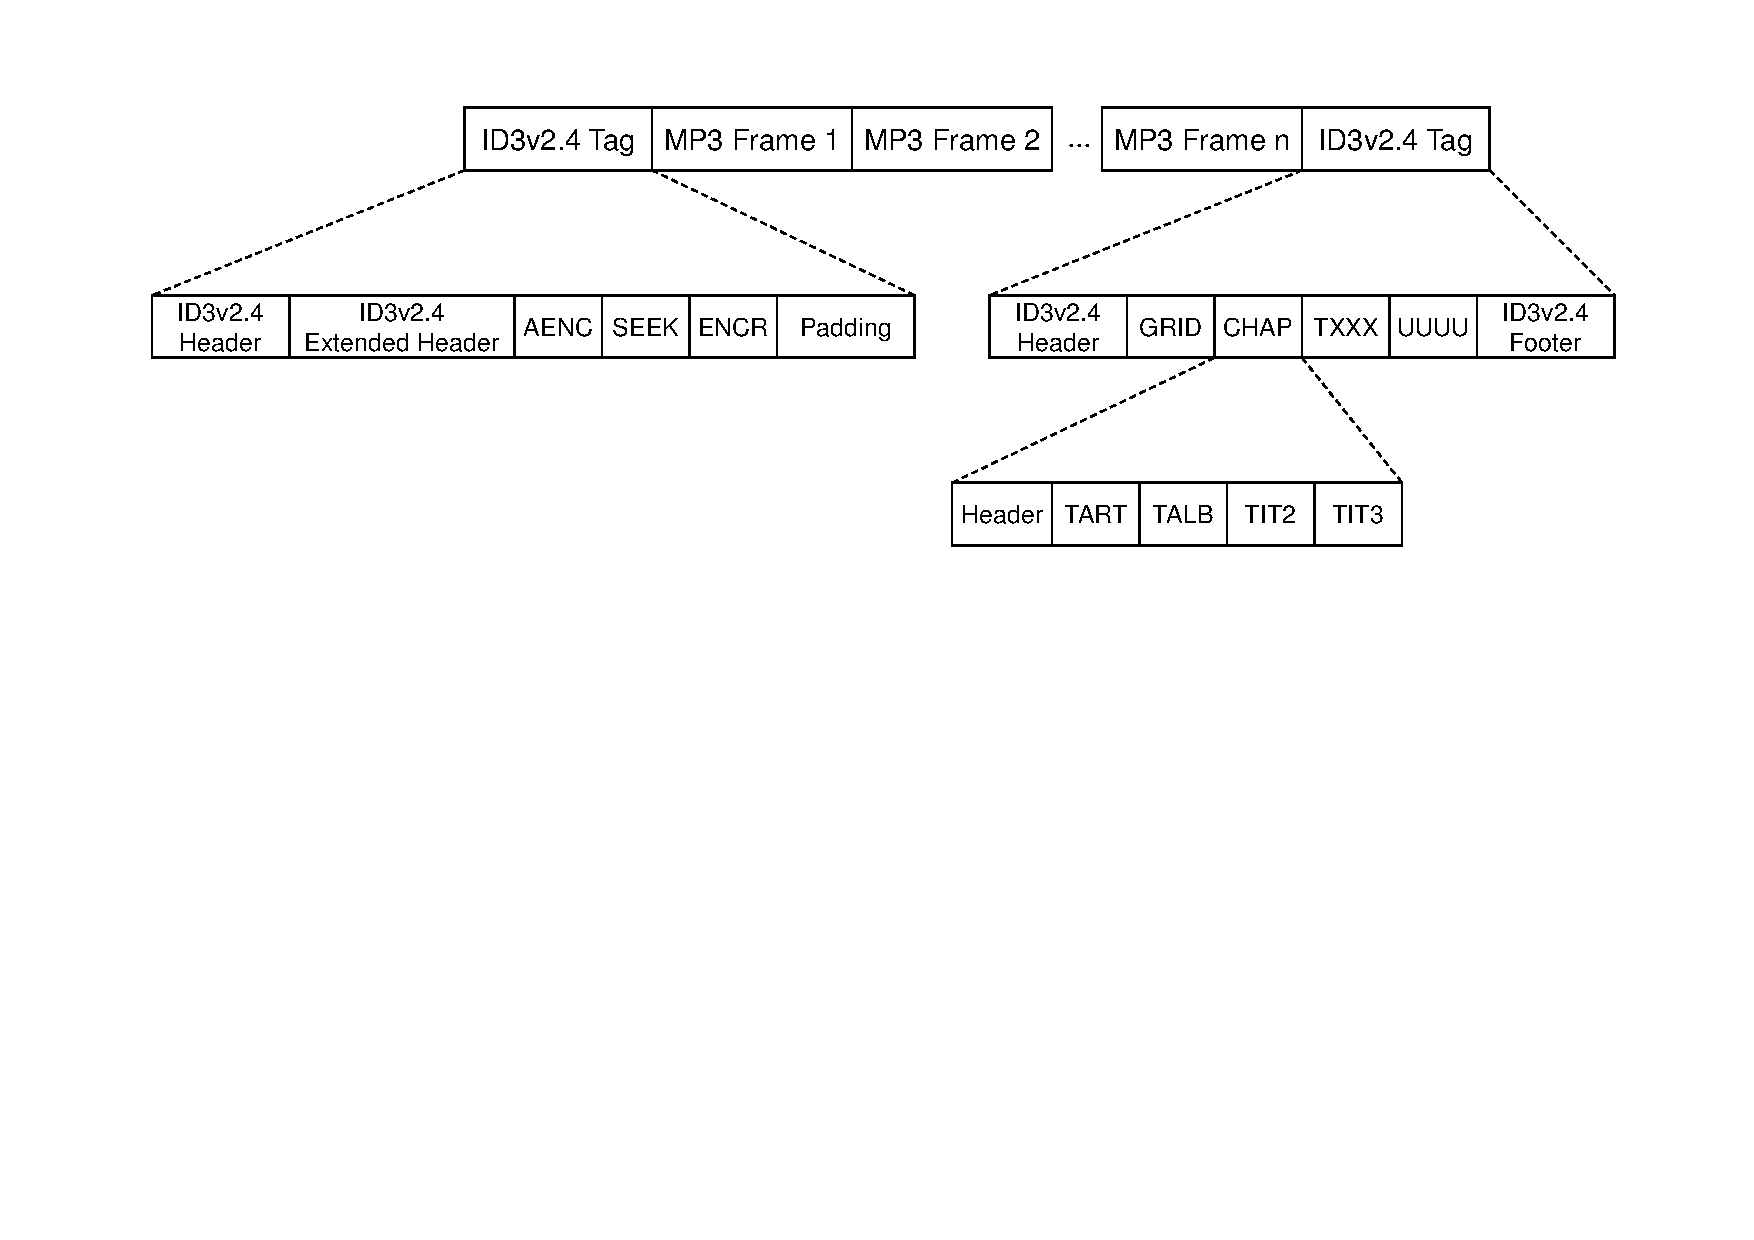
\includegraphics[width=1.00\textwidth]{Figures/Part_I/I_5_Example2.pdf}
	\caption{Example 2: MP3 file with two ID3v2.4 tags}
	\label{fig:Example1MP3filewithtwoID3tags}
\end{figure}

The two ID3v2.4 tags are virtually connected by a \texttt{SEEK} frame. Both have several specialties described in \cite{MetadataCompendium}.

%-----------------------------------------------------------------------------------------------
%		Example 3: MP3 Media Stream with periodic ID3v2.3 Tags
%-----------------------------------------------------------------------------------------------

\section{Example 3: MP3 Media Stream with periodic ID3v2.3 Tags}
\label{sec:Example3MP3FileWithID3v23AndID3v11}

The following figure shows the third example, an MP3 media stream with wildly scattered or periodic ID3v2.3 \TERMtag{}s. The figure shows that start of listening to the stream may also be in the middle of an MP3 block:

\begin{figure}[H]
	\centering
	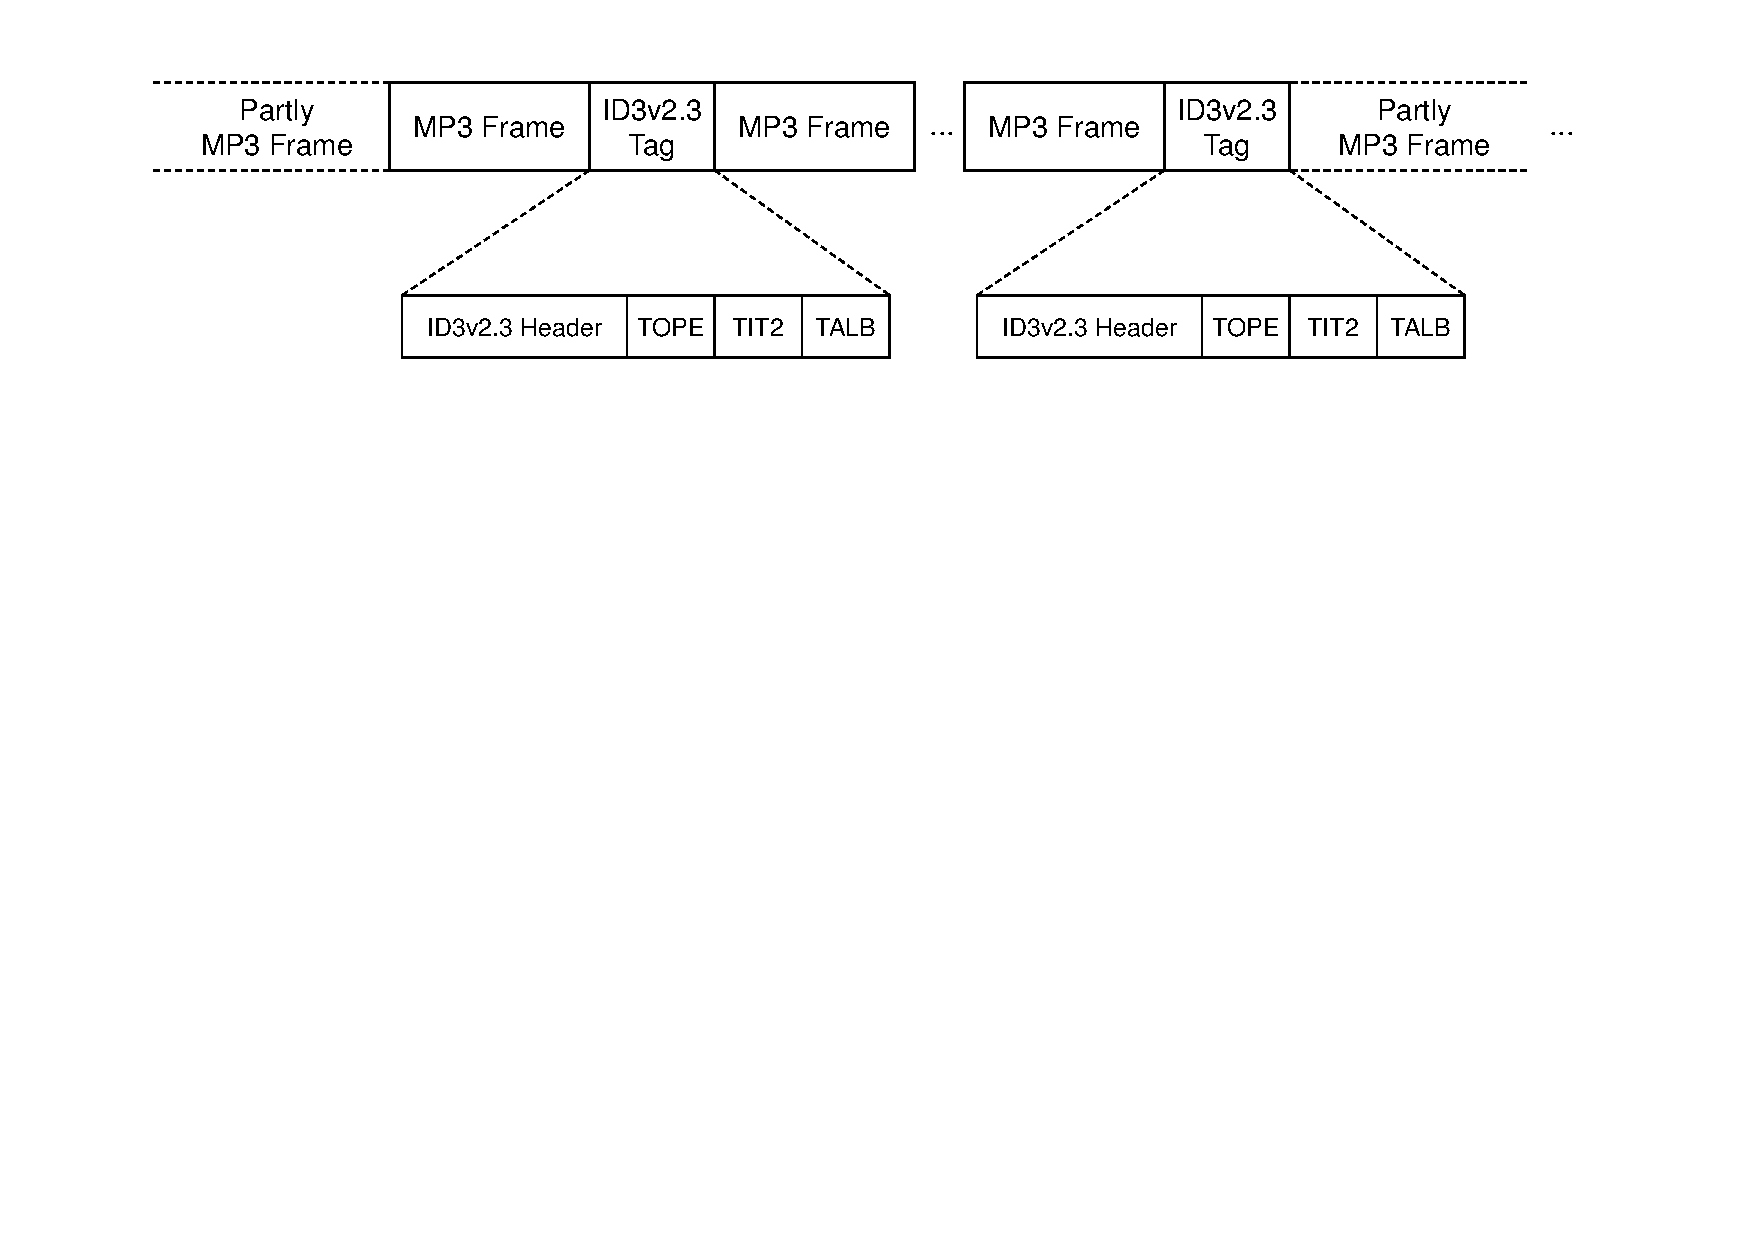
\includegraphics[width=1.00\textwidth]{Figures/Part_I/I_5_Example3.pdf}
	\caption{Example 3: MP3 Media Stream with periodic ID3v2.3 Tags}
	\label{fig:Example3MP3filewithtwoID3tags}
\end{figure}

%-----------------------------------------------------------------------------------------------
%		Example 4: Ogg Bitstream with Theora and VorbisComment
%-----------------------------------------------------------------------------------------------

\section{Example 4: Ogg Bitstream with Theora and VorbisComment}
\label{sec:Example4MP3FileWithID3v23AndID3v11}

The following figure shows the fourth example, an Ogg bitstream that contains Theora payload data with a corresponding vorbis comment:

\begin{figure}[H]
	\centering
	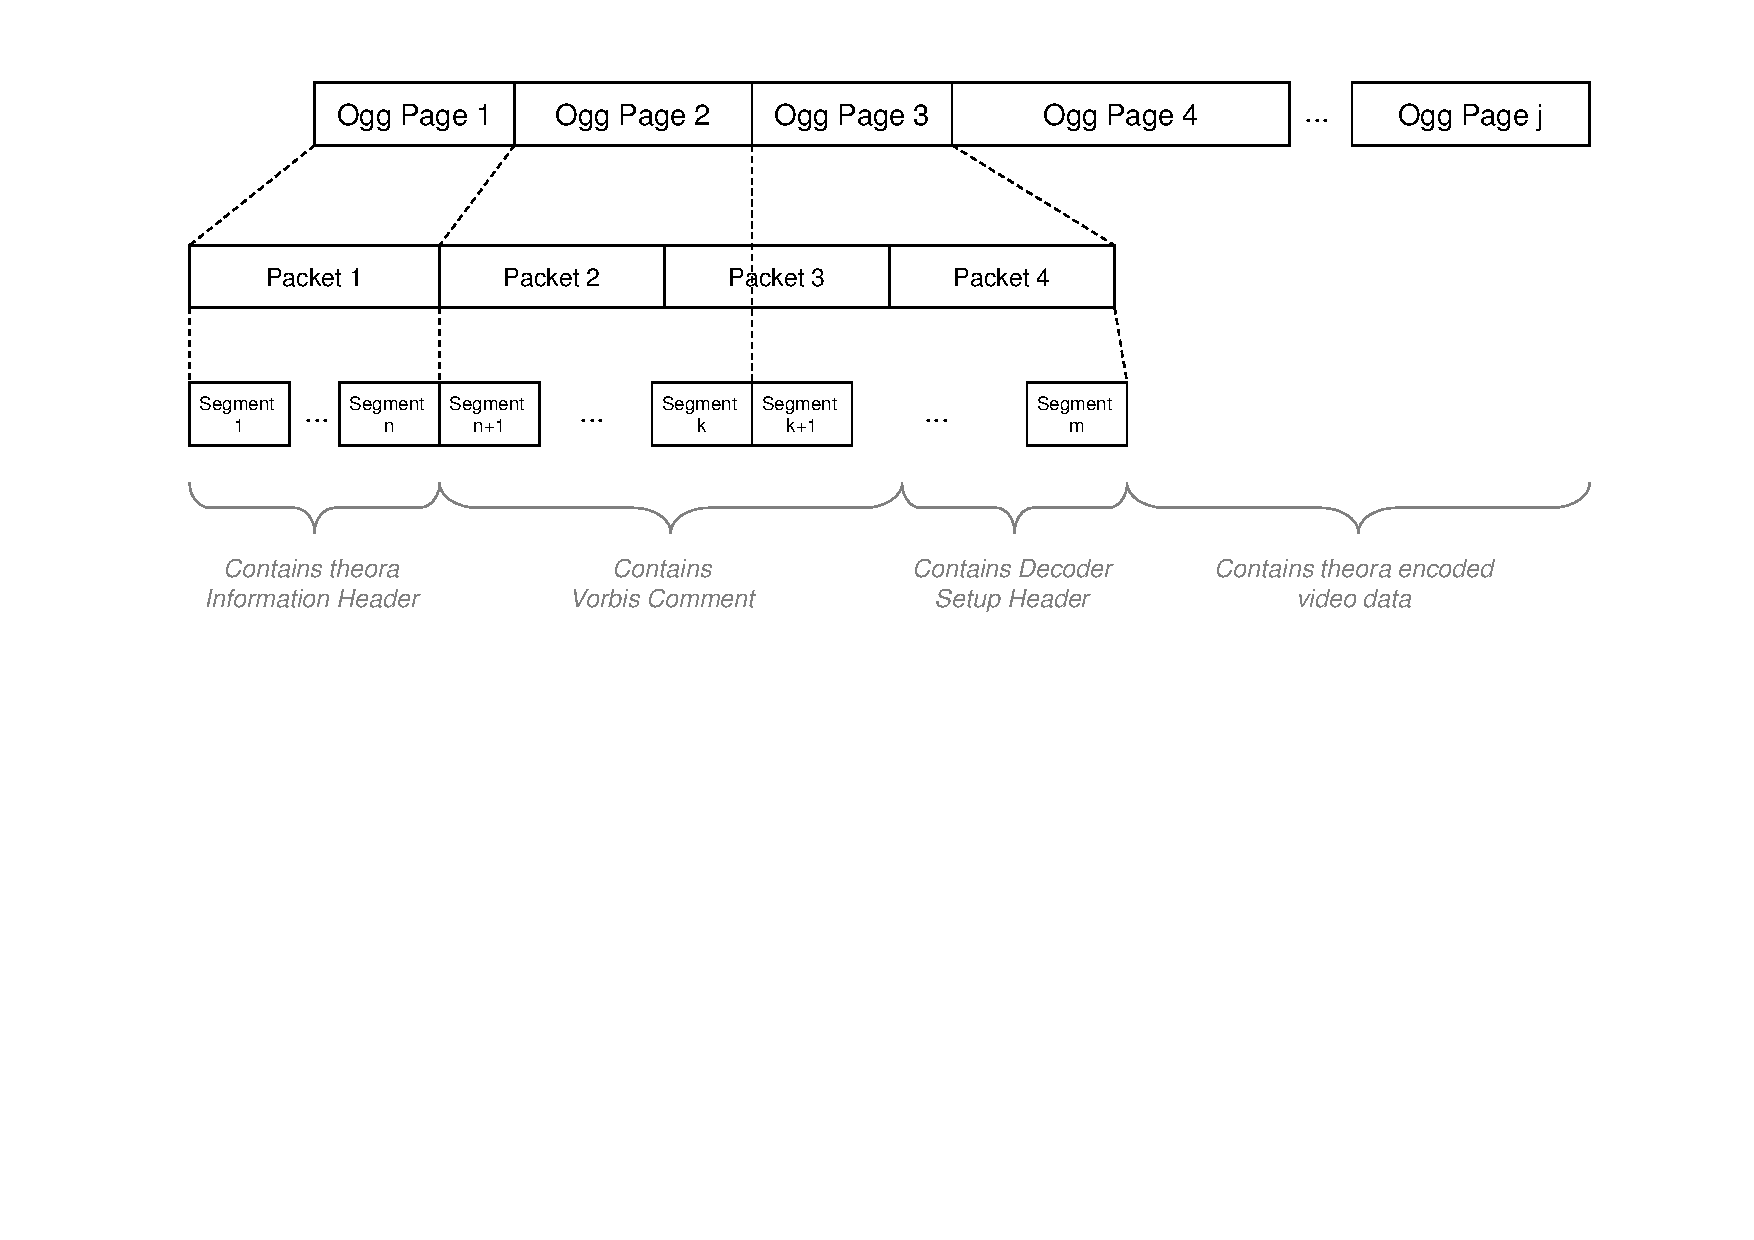
\includegraphics[width=1.00\textwidth]{Figures/Part_I/I_5_Example4.pdf}
	\caption{Example 4: Ogg Bitstream with Theora and VorbisComment}
	\label{fig:Example4MP3filewithtwoID3tags}
\end{figure}

The example is complex on first sight. In an Ogg bitstream, physical and logical structure are not necessarily the same. The physical structure is built by pages, packets and segments, while the logical structure is the structure of the wrapped data. We took theora video data as an example, but its basically arbitrary, as the codec does not really matter. What matters is where the Vorbis Comment, one of the supported data formats, is stored. This unfortunately depends on the embedded codec. In this example, the vorbis comment starts in the second page and spans over two packets. The second of these packets spans over two Ogg pages.

% %-----------------------------------------------------------------------------------------------
% %		Example 5: TIFF RGB image file
% %-----------------------------------------------------------------------------------------------

% \section{Example 5: TIFF RGB image file with Exif IFD}
% \label{sec:Example5MP3FileWithID3v23AndID3v11}

% An example RGB image TIFF file with an Exif IFD is modelled in the following figure:\footnote{The example is based on the figure of \cite{ExifSpec}, page 9.}

% \begin{figure}[H]
% 	\centering
% 	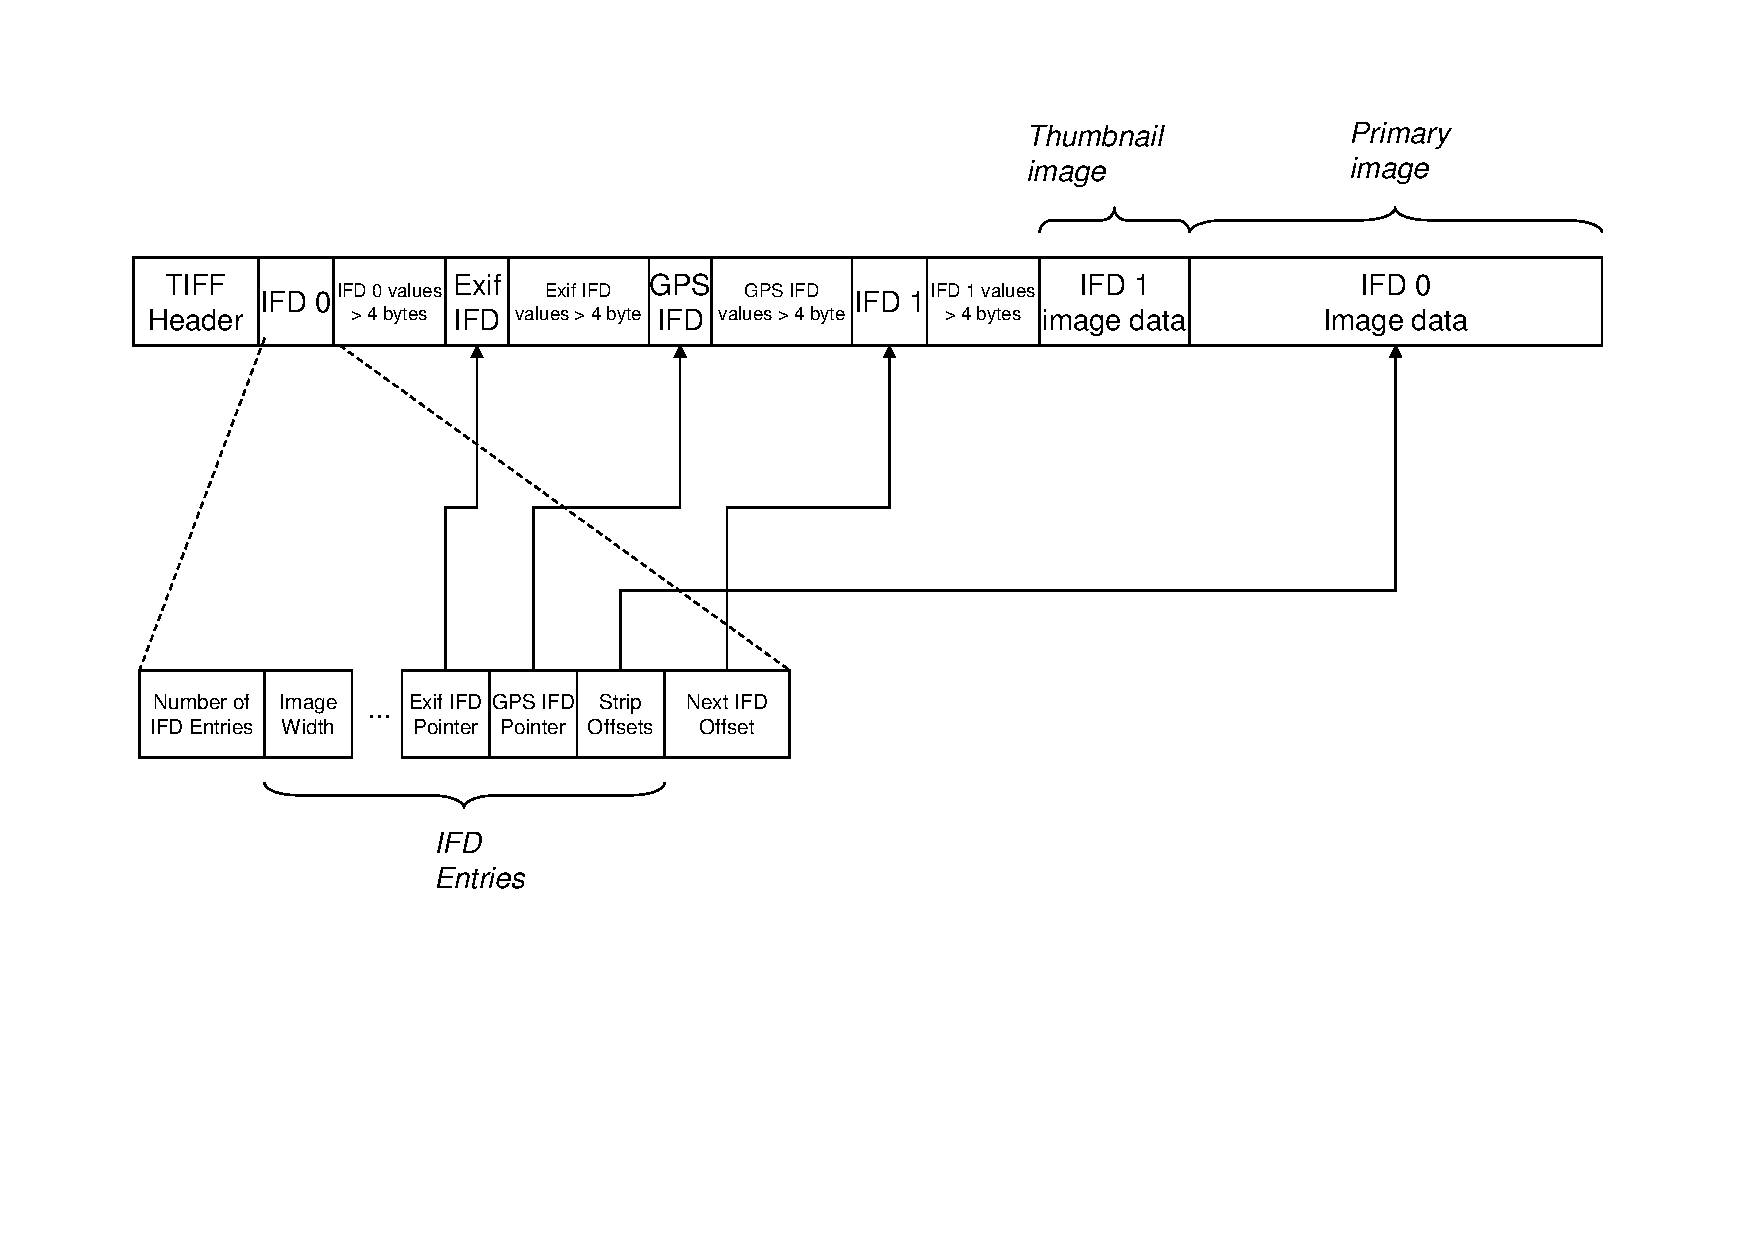
\includegraphics[width=1.00\textwidth]{Figures/Part_I/I_5_Example5.pdf}
% 	\caption{Example 5: TIFF RGB image file with Exif IFD}
% 	\label{fig:Example5MP3filewithtwoID3tags}
% \end{figure}

% Note that Exif is \emph{not a supported format} for \LibName{} currently. However, the presence of an Exif IFD must not be a problem for \LibName{}, of course.

% The example contains two image data parts, in this example stored after each other. The first image part is just a thumbnail image while the second one stores the real image data. The figure shows the pointered structure of the file as IFD fields often point to a byte offset in the file where the actual data is stored.

% %-----------------------------------------------------------------------------------------------
% %		Example 6: RIFF WAVE File
% %-----------------------------------------------------------------------------------------------

% \section{Example 6: RIFF WAVE File}
% \label{sec:Example6MP3FileWithID3v23AndID3v11}

% An example RIFF file with WAVE sound contents is shown in the following figure:

% \begin{figure}[H]
% 	\centering
% 	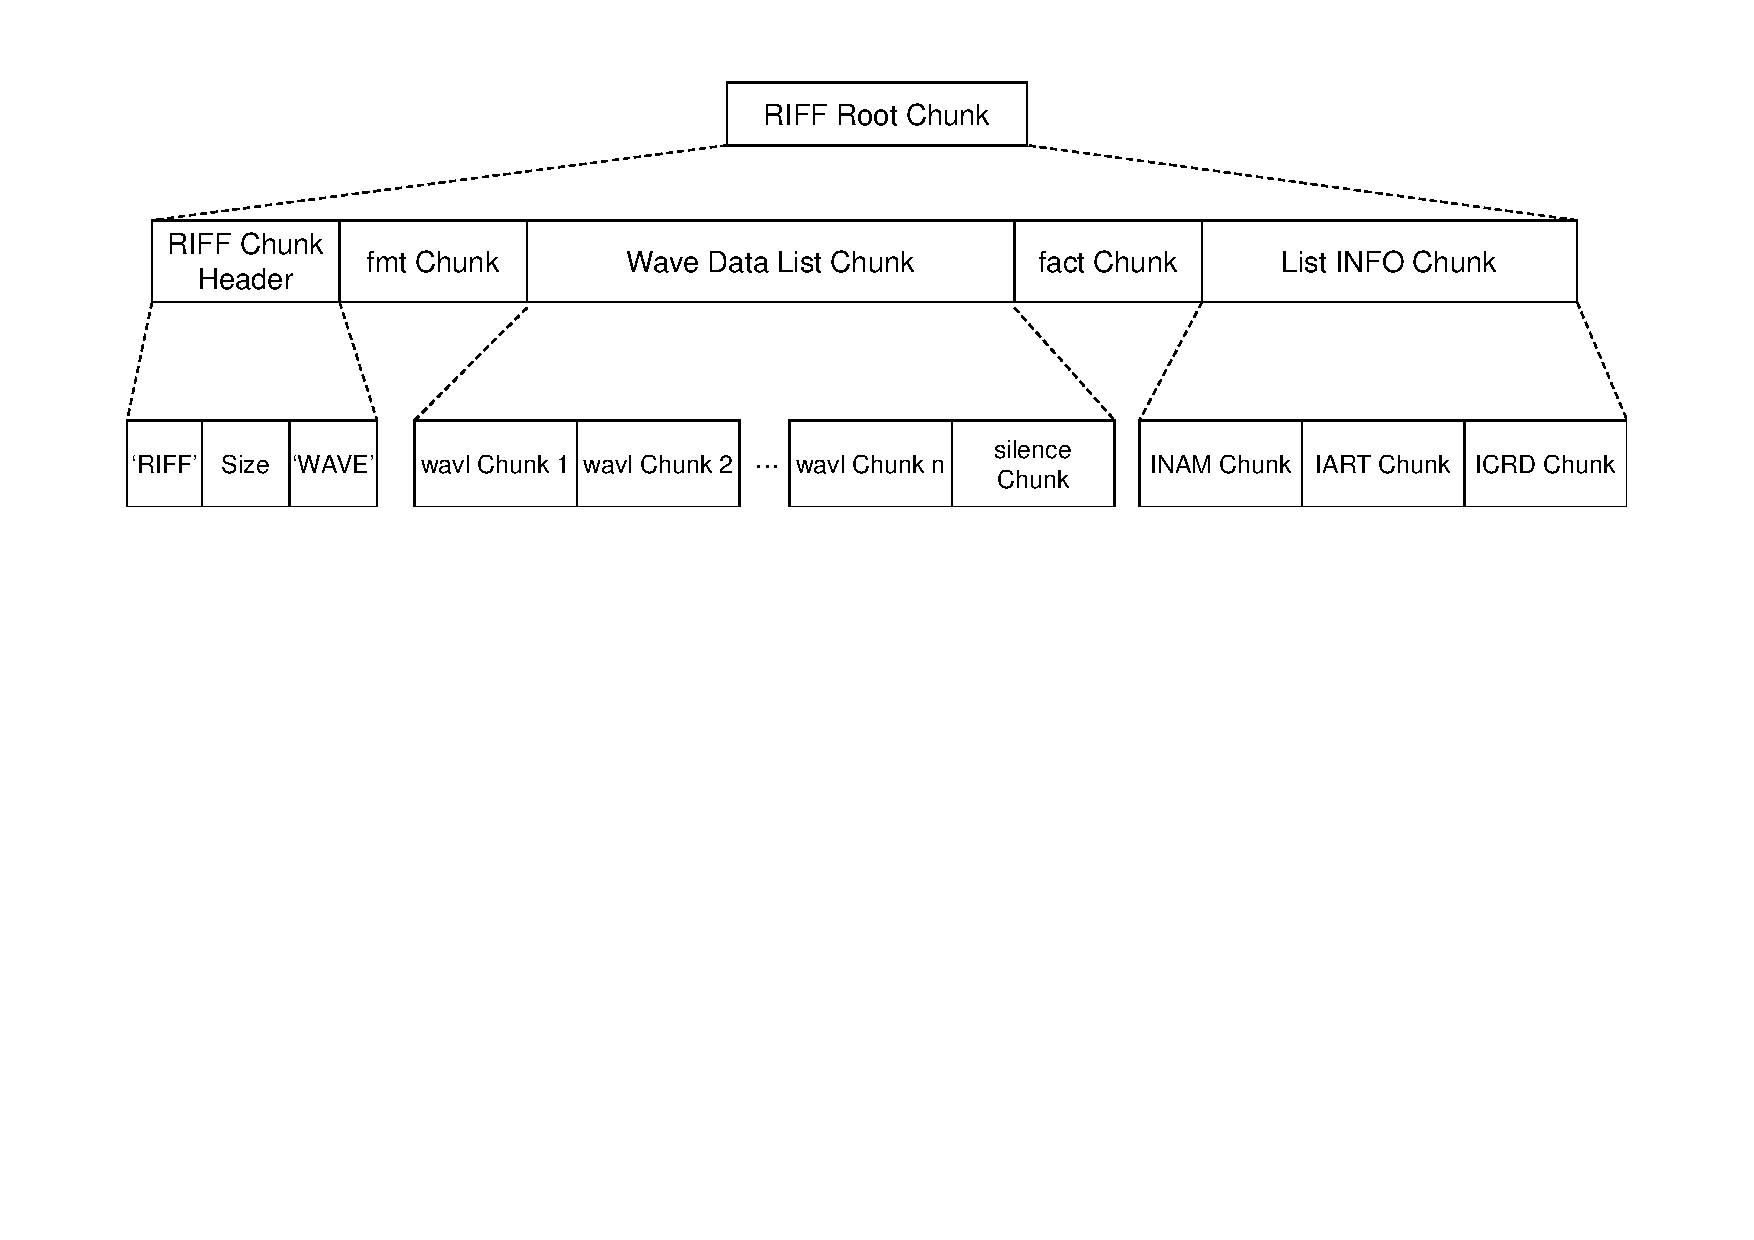
\includegraphics[width=1.00\textwidth]{Figures/Part_I/I_5_Example6.pdf}
% 	\caption{Example 6: RIFF WAVE File}
% 	\label{fig:Example6MP3filewithtwoID3tags}
% \end{figure}

% The top-level root chunk contains a fact chunk, a format chunk, a list of wave data chunks and finally a \texttt{LIST} info chunk in its payload. The \texttt{LIST} info chunk can be considered as \TERMtagBasic{}. It contains \texttt{INAM}, \texttt{IART} and \texttt{ICRD} sub-chunks.

% %-----------------------------------------------------------------------------------------------
% %		Example 7: QuickTime File
% %-----------------------------------------------------------------------------------------------

% \section{Example 7: QuickTime File}
% \label{sec:Example7MP3FileWithID3v23AndID3v11}

% An example QuickTime file is shown in the following figure:

% \begin{figure}[H]
% 	\centering
% 	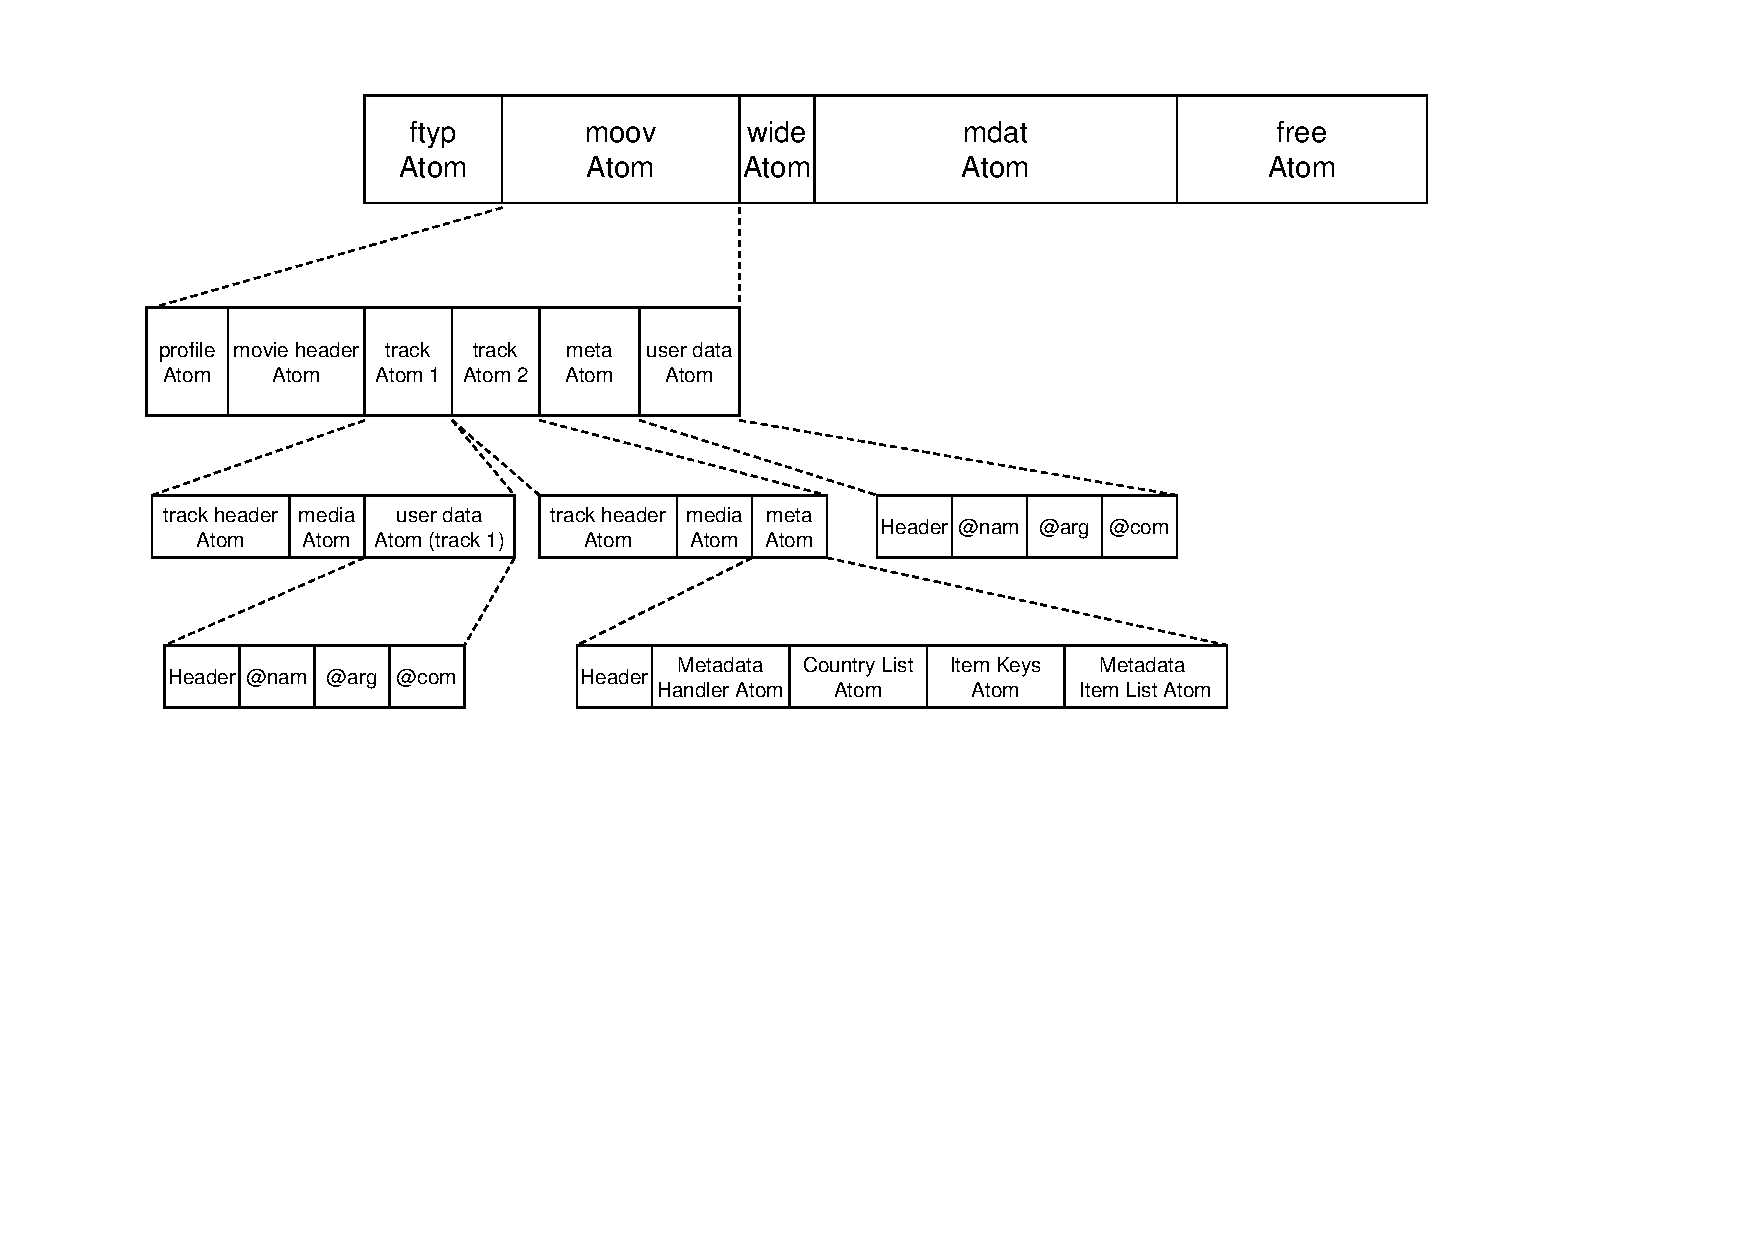
\includegraphics[width=1.00\textwidth]{Figures/Part_I/I_5_Example7.pdf}
% 	\caption{Example 7: QuickTime File}
% 	\label{fig:Example7MP3filewithtwoID3tags}
% \end{figure}

% A QuickTime file can easily get very complex. The example contains the \texttt{ftyp}, \texttt{moov}, \texttt{mdat} and \texttt{free} atoms as top-level atoms. The \texttt{mdat} atom contains the media data and is not further detailed in the example. It is preceded by a wide atom to enable easy extension to a header indicating more than $2^{32}$ bytes media atom size.

% The example defines two tracks in the movie atom. One of these contains a user data atom which contains key-value metadata. The other track contains the QuickTime \texttt{meta} atom also defining metadata, but in a different way.

% The example shows that the \texttt{moov} atom itself additionally contains a \texttt{meta} and user data atom describing the whole file.

% %-----------------------------------------------------------------------------------------------
% %		Example 8: Matroska File
% %-----------------------------------------------------------------------------------------------

% \section{Example 8: Matroska File}
% \label{sec:Example8MP3FileWithID3v23AndID3v11}

% An example Matroska file is shown in the following figure:

% \begin{figure}[H]
% 	\centering
% 	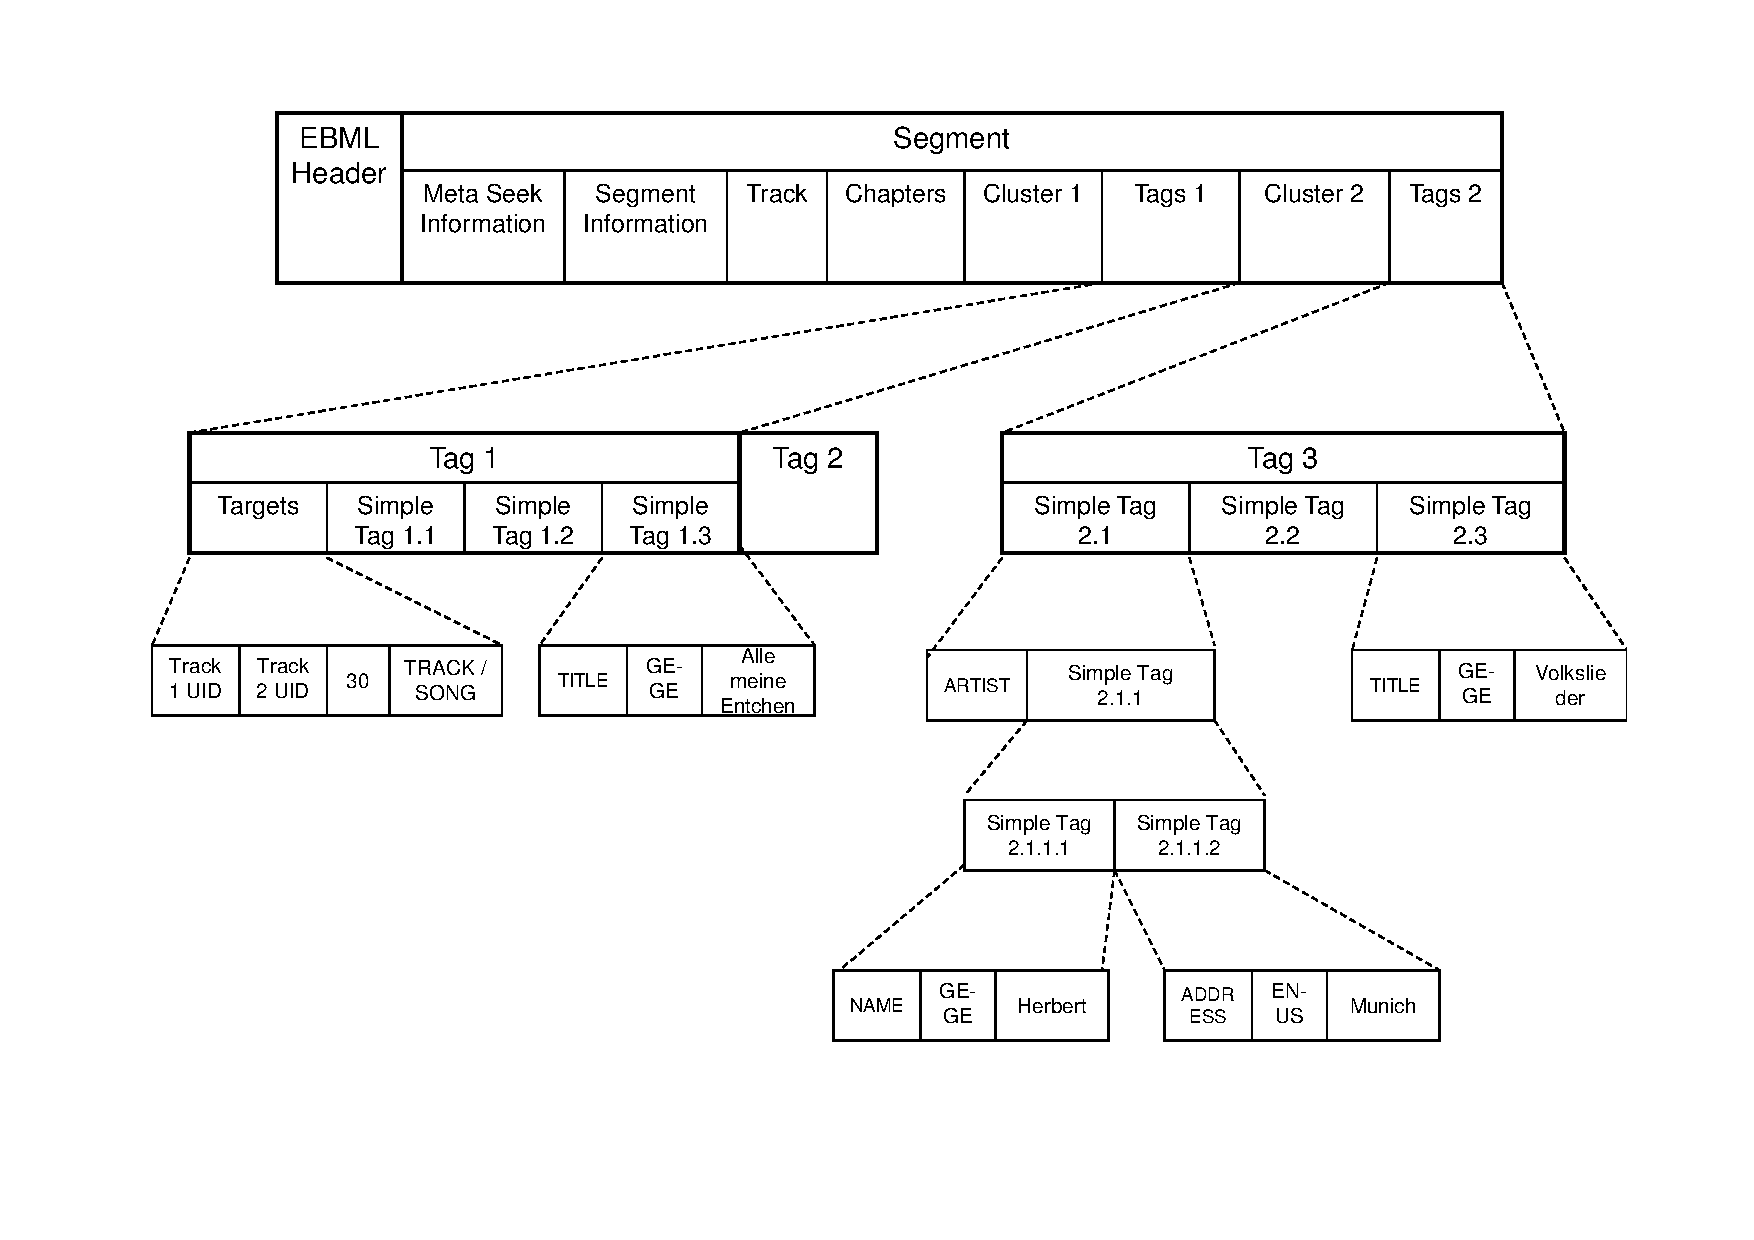
\includegraphics[width=1.00\textwidth]{Figures/Part_I/I_5_Example8.pdf}
% 	\caption{Example 8: Matroska File}
% 	\label{fig:Example8MP3filewithtwoID3tags}
% \end{figure}

% The example has two Cluster elements that store the actual media data. These are not further detailed in the example. The metadata in the example is complex: There are two top-level Tags elements, the first one contains two Tag elements, the second one only a single Tag element. Each of the Tag elements has child SimpleTag elements. The first Tag contains a Targets sub-element that points to two tracks of the file. Tag 3 only contains SimpleTags. However, the first SimpleTag contains nested SimpleTags.

% %-----------------------------------------------------------------------------------------------
% %		Example 9: Arbitrary XML
% %-----------------------------------------------------------------------------------------------

% \section{Example 9: Arbitrary XML}
% \label{sec:Example9MP3FileWithID3v23AndID3v11}

% \LibName{} is required to handle arbitrary XML data, too. The following short file is taken as an example:

% \begin{lstlisting}
% <?xml version="1.0" encoding="UTF-8"?>
% <!DOCTYPE ComponentConfiguration [ 

% <!ELEMENT ComponentDescriptor (Service+)>

% <!ATTLIST id NAME CDATA #REQUIRED>

% ]> 
% <cconf:ComponentConfiguration
% xmlns:cconf="www.easytag.de/XMLSchema_v1_0"
% 	xmlns:xsi="http://www.w3.org/2001/XMLSchema-instance"
% 	xsi:schemaLocation="www.easytag.de/XMLSchema_v1_0 ComponentConfiguration.xsd">
% 	<ComponentDescriptor id="a">
% 		<ProviderPath>bin/</ProviderPath>
% 		<Service>
% 			<Interface>de.je.registry.export.compdummies.a.export.TestInterfaceCompA1</Interface>
% 			<Provider>de.je.registry.compdummies.a.impl.TestImplCompA1</Provider>
% 		</Service>
% 		<Service>
% 			<Interface>de.je.registry.export.compdummies.a.export.TestInterfaceCompA2</Interface>
% 			<Provider>de.je.registry.compdummies.a.impl.TestImplCompA2</Provider>
% 		</Service>
% 	</ComponentDescriptor>
% 	<ComponentDescriptor id="b">
% 		<ProviderPath>bin/</ProviderPath>
% 		<Service>
% 			<Interface>de.je.registry.export.compdummies.b.export.TestInterfaceCompB1</Interface>
% 			<Provider>de.je.registry.compdummies.b.impl.TestImplCompB1</Provider>
% 		</Service>
% 	</ComponentDescriptor>
% 	<ComponentDescriptor id="c">
% 		<ProviderPath>bin/</ProviderPath>
% 		<Service>
% 			<Interface>de.je.registry.export.compdummies.c.export.TestInterfaceCompC1</Interface>
% 			<Provider>de.je.registry.compdummies.c.impl.TestImplCompC1</Provider>
% 		</Service>
% 	</ComponentDescriptor>
% 	<ComponentDescriptor id="d">
% 		<ProviderPath>bin/</ProviderPath>
% 		<Service>
% 			<Interface>de.je.registry.export.compdummies.d.export.XYZ</Interface>
% 			<Provider>de.je.registry.compdummies.d.impl.XYZImpl</Provider>
% 		</Service>
% 	</ComponentDescriptor>
% </cconf:ComponentConfiguration>
% \end{lstlisting}

% The example contains most XML elements: DTD, Elements, attributes, namespaces and of course the XML header.

% %-----------------------------------------------------------------------------------------------
% %		Example 10: Arbitrary XHTML with Meta Elements and RDFa
% %-----------------------------------------------------------------------------------------------

% \section{Example 10: Arbitrary XHTML with Meta Elements and RDFa}
% \label{sec:Example10MP3FileWithID3v23AndID3v11}

% \LibName{} is required to handle arbitrary XHTML data, and especially XHTML meta elements and embedded RDFa. All of this is contained in the following example:

% \begin{lstlisting}
% <?xml version="1.0" encoding="UTF-8"?>
% <!DOCTYPE html
%   PUBLIC "-//W3C//DTD XHTML 1.0 Transitional//EN"
%   "http://www.w3.org/TR/xhtml1/DTD/xhtml1-transitional.dtd">
% <html xmlns="http://www.w3.org/1999/xhtml"
%     version="XHTML+RDFa 1.0"
% 	 xmlns:biblio="http://example.org/"
%     xmlns:dc="http://purl.org/dc/elements/1.1/"
%     xmlns:cal="http://www.w3.org/2002/12/cal/ical#"
%  	 xmlns:foaf="http://xmlns.com/foaf/0.1/"
%     xml:lang="en"
%      profile="http://example.org/profil.html">
%   <head>
%     <title>Books by Marco Pierre White</title>
%     <!-- There is no about attribute here which means the predicate dc:creator with object (i.e. value) "Mark Birbeck" refers to the current document as a subject -->
%     <meta property="dc:creator" content="Mark Birbeck" />
%     <!-- Another example of a predicate that expresses a relationship "foaf:topic" to the specified URI. -->
%     <link rel="foaf:topic" href="http://www.formsPlayer.com/#us" />
% 	 <link rel="foaf:primaryTopic" href="#bbq" />
% 	<title>Beschreibung der Seite</title>
% 	<meta name="Typ" scheme="MIME-Type" content="image/svg+xml">
% 	<meta name="author" content="Anna Lyse">
% 	<meta http-equiv="expires" content="Sat , 01 Dec 2001 00:00:00 GMT">
% 	<meta name="keywords" lang="de" content="Ferien , Griechenland ,
% 		Sonnenschein">
% 	<meta name="keywords" lang="en-us" content="vacation , Greece , sunshine">
% 	<meta name="keywords" lang="en" content="holiday , Greece , sunshine">
% 	<meta name="keywords" lang="fr" content="vacances , Gr&egrave;ce , soleil">
% 	<meta http-equiv="content-type" content="text/html; charset=ISO-8859-1">
% 	<meta http-equiv="Content-Script-Type" content="text/javascript">

% 	<meta http-equiv="PICS-Label" content='(PICS-1.1 "http://www.gcf.org/v2.5"
% 		labels on "1994.11.05T08:15-0500"
% 		unti l "1995.12.31T23:59-0000"
% 		for "http://w3c.org/PICS/Overview.html"
% 		ratings ( suds 0.5 density 0 color/hue 1) ) '>
%   </head>
%   <body>
%     I think White's book
%     <!-- Here comes the first subject embedded in a span element. It refers to a specific datatype using typeof. It is described with the predicate dc:title whose object (i.e. value) is
%     the contents of the span element. -->
%     '<span about="urn:ISBN:0091808189" typeof="biblio:book"
%            property="dc:title">
%       Canteen Cuisine
%     </span>'
%     is well worth getting since although it's quite advanced stuff, he
%     makes it pretty easy to follow. You might also like
%     <!-- The second subject whose dc:description is given. -->
%     <span about="urn:ISBN:1596913614" typeof="biblio:book"
%           property="dc:description">
%       White's autobiography
%     </span>.
%     <!-- Another subject -->
%     <p about="#bbq" typeof="cal:Vevent">
%       I'm holding
%       <span property="cal:summary">
%         one last summer barbecue
%       </span>,
%       on
%       <!-- Here the object is not the content of the span attribute but the value of the "content" attribute -->
%       <span property="cal:dtstart" content="2007-09-16T16:00:00-05:00"
%             datatype="xsd:dateTime">
%         September 16th at 4pm
%       </span>.
%     </p>
% </body>
% </html>
% \end{lstlisting}

% The example is not real but constructed from various sources. It contains as much different elements as possible:
% \begin{itemize}
% 	\item Some meta elements with a @name attribute
% 	\item Some meta elements with a @http-equiv attribute
% 	\item A meta element containing PICS metadata. PICS is not directly supported in \Lib{}. However, the generic meta elements must be parsed correctly, no matter what they contain.
% 	\item Some meta elements using specific namespaces or profiles
% 	\item RDFa metadata
% \end{itemize}

% %-----------------------------------------------------------------------------------------------
% %		Example 11: An RDF/XML File
% %-----------------------------------------------------------------------------------------------

% \section{Example 11: An RDF/XML File}
% \label{sec:Example11MP3FileWithID3v23AndID3v11}

% \begin{lstlisting}
% <?xml version="1.0" encoding="UTF-8"?>
% <rdf:RDF xmlns:rdf="http://www.w3.org/1999/02/22-rdf-syntax-ns#"
%          xmlns:pcv="http://prismstandard.org/namespaces/pcv/1.0/"
%          xmlns:dc="http://purl.org/dc/elements/1.1/"
%          xml:base="http://travel.example.com/"
%          xmlns:s="http://example.org/students/vocab#"
%          xmlns:exterms="http://www.example.org/terms/">

%   <rdf:Description rdf:about="/2000/08/Corfu.jpg">
%     <dc:identifier rdf:resource="/content/2357845" />
%     <dc:creator>
%       <pcv:Descriptor rdf:about="/emp3845">
%         <pcv:label>John Peterson</pcv:label>
%       </pcv:Descriptor>
%     </dc:creator>
%     <dc:coverage>
%       <pcv:Descriptor
%           rdf:about="http://prismstandard.org/vocabs/ISO-3166/GR">
%         <pcv:label xml:lang="en">Greece</pcv:label>
%         <pcv:label xml:lang="fr">Grece</pcv:label>
%       </pcv:Descriptor>
%     </dc:coverage>
%   </rdf:Description>

%   <rdf:Description rdf:about="/2000/08/Corfu.jpg">
%     <dc:identifier rdf:resource="/content/2357845" />
%     <dc:creator>
%     	Michael
%     </dc:creator>
%   </rdf:Description>
  
%    <rdf:Description rdf:about="http://example.org/courses/6.001">
%       <s:students rdf:parseType="Collection">
%          <rdf:Description rdf:about="http://example.org/students/Amy"/>
%          <rdf:Description rdf:about="http://example.org/students/Mohamed"/>
%          <rdf:Description rdf:about="http://example.org/students/Johann"/>
%       </s:students>
%    </rdf:Description>

%   <rdf:Description rdf:about="http://www.example.com/2002/04/products#item10245">
%      <exterms:weight rdf:parseType="Resource">
%        <rdf:value rdf:datatype="&xsd;decimal">2.4</rdf:value>
%        <exterms:units rdf:resource="http://www.example.org/units/kilograms"/>
%      </exterms:weight>
%   </rdf:Description>

% </rdf:RDF>
% \end{lstlisting}

% The example contains several rdf:Description elements, even two referring to the same subject. We also have applications of the rdf:parseType, rdf:datatype and rdf:resource attributes. There are also some nested descriptions.

% %-----------------------------------------------------------------------------------------------
% %		Example 12: An XMP File
% %-----------------------------------------------------------------------------------------------

% \section{Example 12: An XMP File}
% \label{sec:Example12MP3FileWithID3v23AndID3v11}

% The following listing shows the XMP reference example:

% \begin{lstlisting}
% <?xpacket begin='?' id='W5M0MpCehiHzreSzNTczkc9d'?>
% <x:xmpmeta xmlns:x='adobe:ns:meta/' x:xmptk='XMPTk 2.8'>

% <rdf:RDF 
% 	xmlns:rdf='http://www.w3.org/1999/02/22-rdf-syntax-ns#' 
% 	xmlns:iX='http://ns.adobe.com/iX/1.0/'>

% 	<rdf:Description about=''
% 		xmlns:xmp='http://ns.adobe.com/xap/1.0/' 
% 		xmp:Author='Jane Doe'
% 		xmp:BaseURL='http://mydoc'
% 		xmp:CreateDate='2001-08-13T10:42:24Z'
% 		xmp:CreatorTool='Microsoft Visual C++ for Windows'
% 		xmp:Format='text/xml'
% 		xmp:MetadataDate='2001-08-13T10:42:24Z'
% 		xmp:ModifyDate='2001-08-13T11:02:13Z'
% 		xmp:Nickname='sample'>
    
% 		<xmp:Advisory>
% 			<rdf:Bag>    
%  				<rdf:li>http://purl.org/dc/elements/1.1/ format</rdf:li>
% 				<rdf:li>http://ns.adobe.com/xap/1.0/xap/g/ NumberOfColors</rdf:li>
% 				<rdf:li>http://ns.adobe.com/xap/1.0/xap/g/img/ Resolution/stRes:units</rdf:li>
% 			</rdf:Bag>
% 		</xmp:Advisory>
  
% 		<xmp:Authors>  
% 			<rdf:Seq>
% 				<rdf:li>Jane Doe</rdf:li>
% 				<rdf:li>John Doe</rdf:li>
% 				<rdf:li>Jack Doe</rdf:li>
% 			</rdf:Seq>
% 		</xmp:Authors>
% 		<xmp:Description>
% 			<rdf:Alt>
% 				<rdf:li xml:lang='en'>This document is a sample XML file</rdf:li>
% 				<rdf:li xml:lang='fr'>Ce document est un fichier d`exemple XML</rdf:li>
% 				<rdf:li xml:lang='de'>Dieses Dokument ist eine XML Beispieldatei</rdf:li>
% 			</rdf:Alt>
% 		</xmp:Description>
  
% 		<xmp:Keywords>
% 			<rdf:Bag>
% 				<rdf:li>XMP</rdf:li>
% 				<rdf:li>Core</rdf:li>
% 				<rdf:li>Schema</rdf:li>
% 				<rdf:li>sample</rdf:li>
% 			</rdf:Bag>
% 		</xmp:Keywords>
% 		<xmp:Locale>
% 			<rdf:Bag>
% 				<rdf:li>en</rdf:li>
% 				<rdf:li>fr</rdf:li>
% 				<rdf:li>de</rdf:li>
% 			</rdf:Bag>
% 		</xmp:Locale>
  
% 		<xmp:Title>
% 			<rdf:Alt>
% 				<rdf:li xml:lang='en'>XMP Core Schema Example</rdf:li>
% 				<rdf:li xml:lang='fr'>XMP Core Schema Exemple</rdf:li>
% 				<rdf:li xml:lang='de'>XMP Core Schema Beispiel</rdf:li>
% 			</rdf:Alt>
% 		</xmp:Title>
  
% 	</rdf:Description>

% </rdf:RDF>

% </x:xmpmeta>
% <?xpacket end='r'?>

% </top_level_element>
% \end{lstlisting}

%###############################################################################################
%###############################################################################################
%
%		File end
%
%###############################################################################################
%###############################################################################################